\usepackage{graphicx, caption}
\usepackage{palatino}
\usepackage[font=scriptsize]{caption}

\definecolor{teal}{cmyk}{0.864, 0.443, 0.000, 0.655}
\definecolor{white}{cmyk}{0.00, 0.00, 0.00, 0.00}

\begin{document}
\begin{poster}
    {
        grid=false,
        eyecatcher=true,
        background=none,
        columns=6,
        headershade=plain,
        headerColorOne=teal,
        headerFontColor=white,
        headerfont=\Large\textsf,
        headerborder=open,
        borderColor=teal,
        textborder=rectangle,
        boxshade=none
    }
    {\includegraphics{images/cs_logo_colour.pdf}}
    {Map of the Internet}
    {Donald Martin}
    {\includegraphics[width=2cm]{images/eyecatcher.png}}

    \headerbox{Motivation}{name=motivation, column=0,row=0, span=3}{
        The Internet is one of the most widely used man-made systems on the planet. So much
        so that former Microsoft CEO, Bill Gates, described the Internet as the ``\emph{town
        square for the village of tomorrow}.'' However, its inner workings are largely unknown
        to the vast majority of its users. Here, I will attempt to shed some light on the
        technical ingenuity behind the Internet.
    }

    \headerbox{Worldwide Connections}{name=worldwide_cxns, column=0, below=motivation, span=3}{
        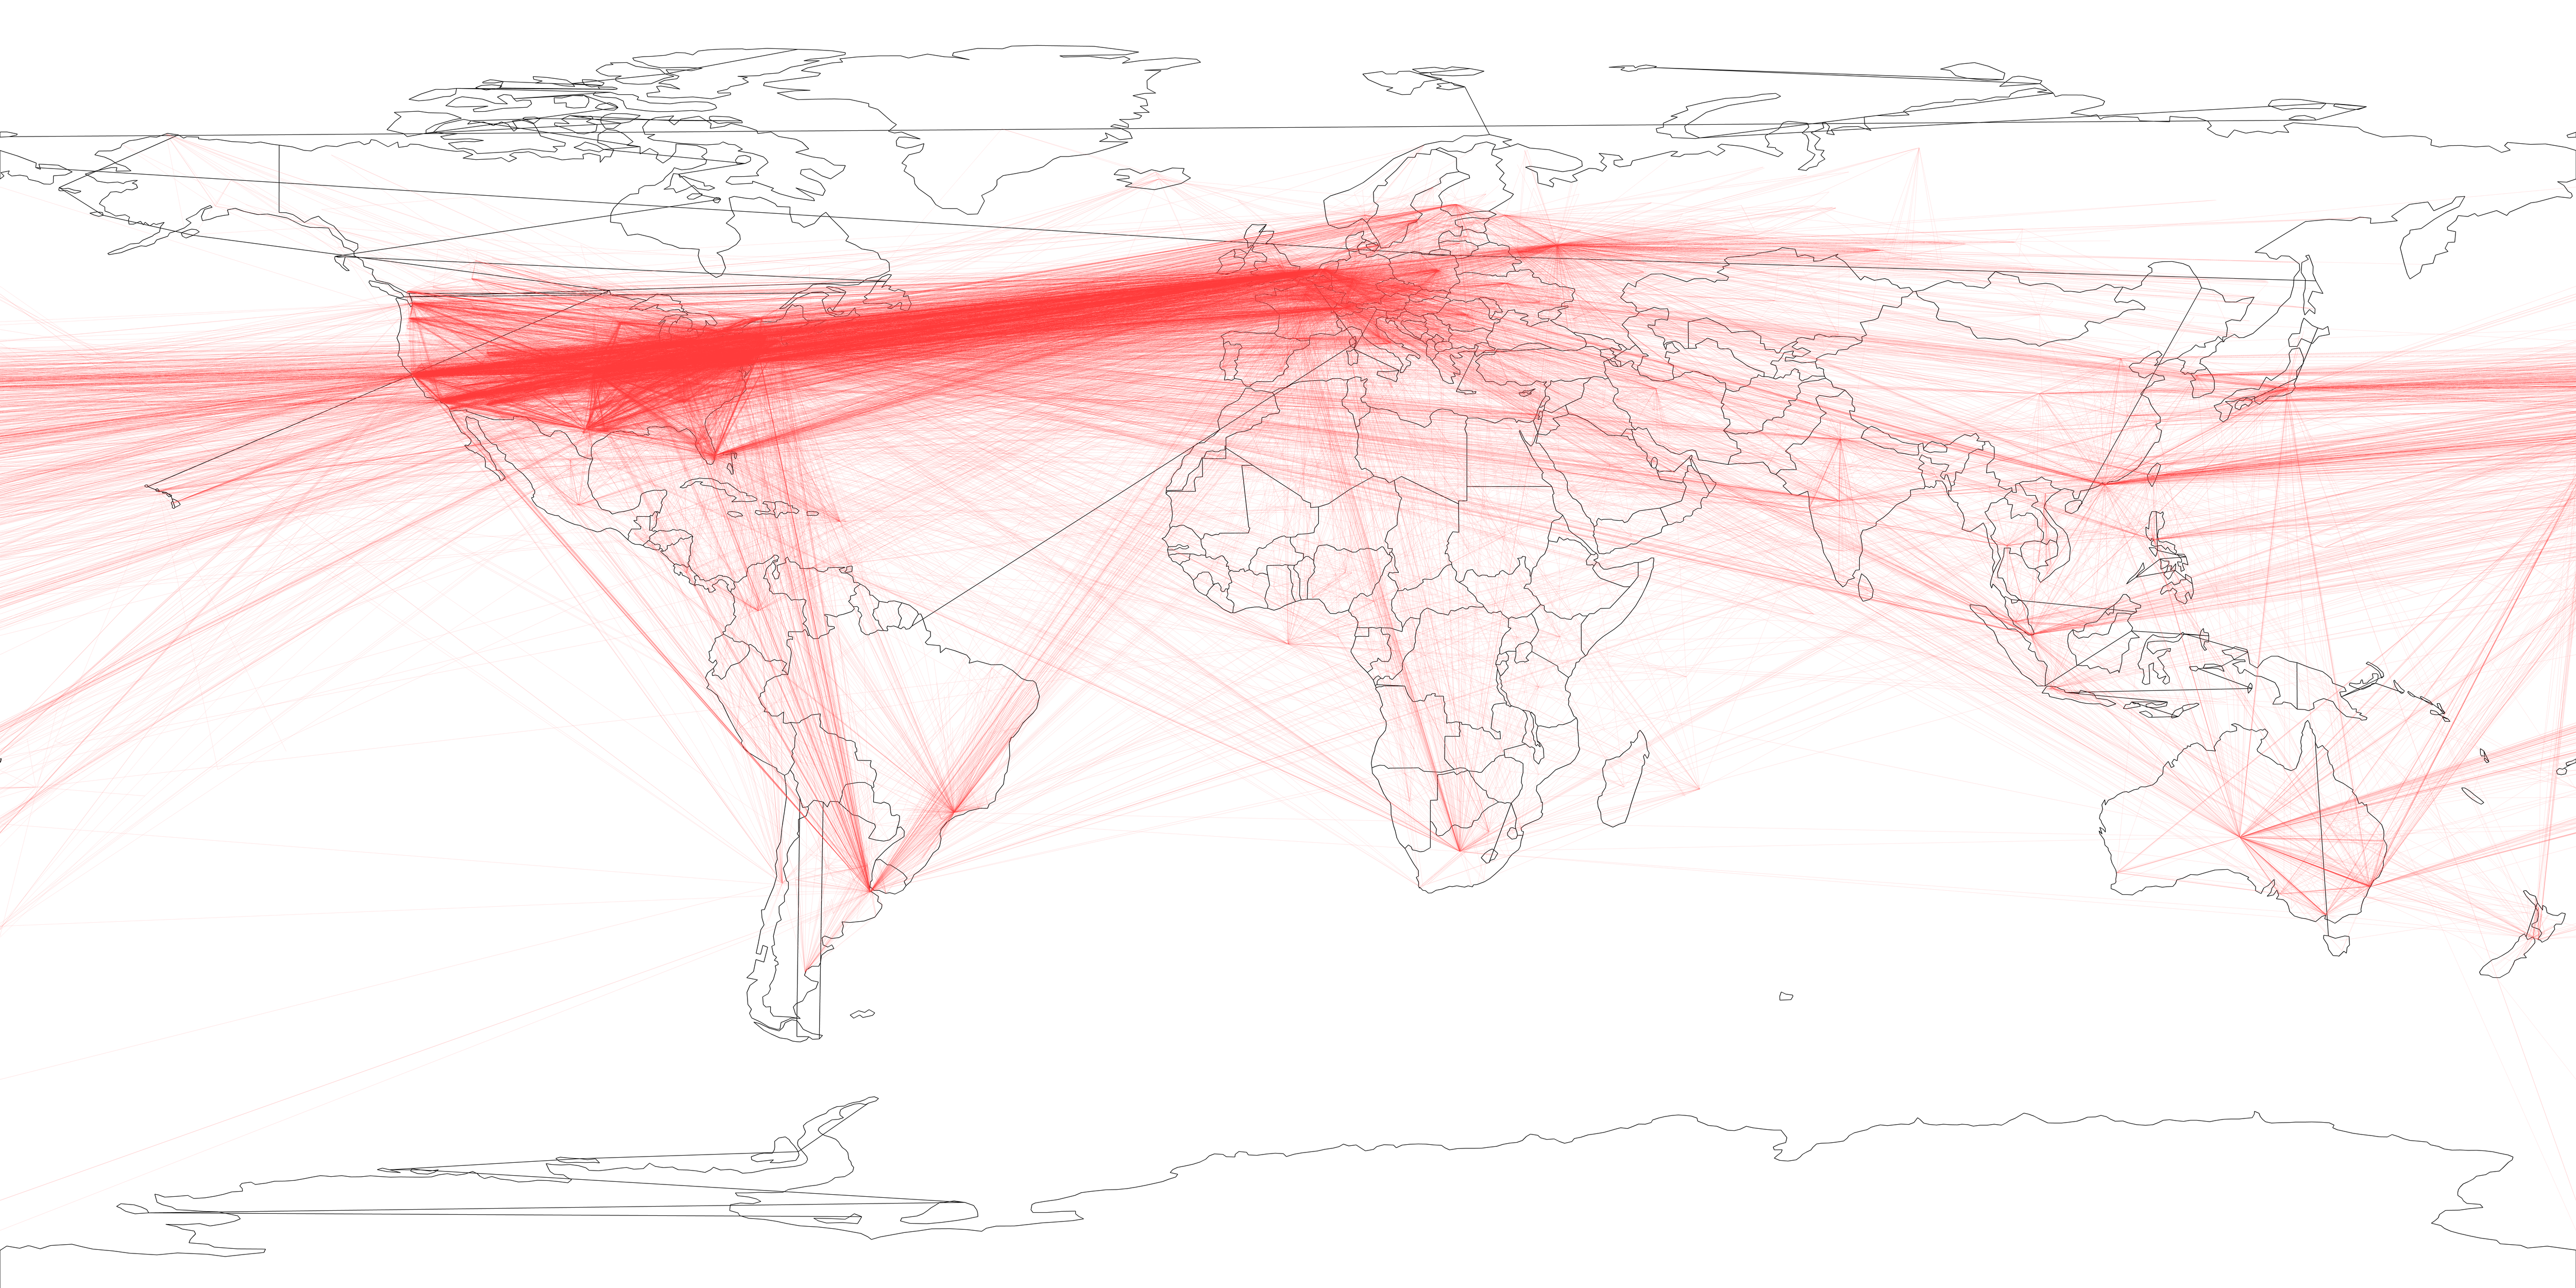
\includegraphics[width=\linewidth]{images/atlas.png}
        \captionof{figure}{Geographical Connections between Autonomous Systems}
        The Internet is foremost a large number of networks of computers working together. Each of these networks is an autonomous system (commonly, these are Internet Service Providers). Above, each autonomous system is represented as a point, based on the geographical location of its headquarters. Connections between autonomous systems are represented as lines. Here, we see a large number of transatlantic connections, showing the extent of Internet connectivity in the developed world, in contrast to Africa which has very few connections to other continents and even fewer autonomous systems.
    }

    \headerbox{The Need for IPv6}{name=need_for_ipv6, column=3,row=0, span=3}{
        \begin{minipage}{0.33\linewidth}
            \includegraphics[width=\linewidth]{images/ipv4_address.png}
            \captionof{figure}{Yearly Visible Addresses}
        \end{minipage}
        \begin{minipage}{0.66\linewidth}
            \includegraphics[width=\linewidth, height=4cm]{images/block_allocs.png}
            \captionof{figure}{Yearly IPv4 Addresses Used}
        \end{minipage}
            $IPV6_NEED_TEXT
    }

    \headerbox{Internet Outages}{name=inet_outages, below=need_for_ipv6, column=3, span=3}{
        \begin{minipage}{0.33\linewidth}
            \includegraphics[width=\linewidth]{$OUTAGE_IMG_1}
            \captionof{figure}{$OUTAGE_CAPT_1}
        \end{minipage}
        \begin{minipage}{0.33\linewidth}
            \includegraphics[width=\linewidth]{$OUTAGE_IMG_2}
            \captionof{figure}{$OUTAGE_CAPT_2}
        \end{minipage}
        \begin{minipage}{0.33\linewidth}
            \includegraphics[width=\linewidth]{$OUTAGE_IMG_3}
            \captionof{figure}{$OUTAGE_CAPT_3}
        \end{minipage}
            $OUTAGES_TEXT
    }

    \headerbox{Other Representations}{below=worldwide_cxns, column=0, span=3}{
        \begin{minipage}{0.33\linewidth}
            \includegraphics[width=0.8\linewidth]{$OTHER_REPR_IMG_1}
            \captionof{figure}{$OTHER_REPR_CAPT_1}
        \end{minipage}
        \begin{minipage}{0.33\linewidth}
            \includegraphics[width=0.8\linewidth]{$OTHER_REPR_IMG_2}
            \captionof{figure}{$OTHER_REPR_CAPT_2}
        \end{minipage}
        \begin{minipage}{0.33\linewidth}
            $OTHER_REPR_TEXT
        \end{minipage}
    }

    \headerbox{Conclusions}{below=inet_outages, column=3, span=3}{
        $CONCLUSION_TEXT
    }
\end{poster}
\end{document}
